\chapter{The Fundamental Group}
\section*{The Fundamental Grupoid}
\subsection*{Construction of the fundamental Grupoid}

\begin{lemma}[Gluing Lemma]
	Let $X,Y \in \ob(\mathsf{Top})$, $(X_\alpha)_{\alpha \in A}$ a finite closed cover of $X$ and $(f_\alpha)_{\alpha \in A}$ a finite family of maps $f_\alpha \in \mathsf{Top}(X_\alpha,Y)$ such that $f_\alpha\vert_{X_\alpha \cap X_\beta} = f_\beta\vert_{X_\alpha \cap X_\beta}$ for all $\alpha,\beta \in A$. Then there exists a unique $f \in \mathsf{Top}(X,Y)$ such that $f\vert_{X_\alpha} = f_\alpha$ for all $\alpha \in A$.
	\label{lem:gluing_lemma}
\end{lemma}

\begin{proof}
	Let $x \in X$. Since $(X_\alpha)_{\alpha \in A}$ is a cover of $X$, we find $\alpha \in A$ such that $x \in X_\alpha$. Define $f(x) := f_\alpha(x)$. This is well defined, since if $x \in X_\alpha \cap X_\beta$ for some $\beta \in A$, we have that $f(x) = f_\beta(x) = f_\alpha(x)$. Clearly $f\vert_{X_\alpha} = f_\alpha$ for all $\alpha \in A$ and $f$ is unique. Let us show continuity. To this end, let $K \subseteq Y$ be closed. Then 
	\begin{align*}
		f^{-1}(K) &= X \cap f^{-1}(K)\\
		&= \bigcup_{\alpha \in A} X_\alpha \cap f^{-1}(K)\\
		&= \bigcup_{\alpha \in A} \del[1]{X_\alpha \cap f^{-1}(K)}\\
		&= \bigcup_{\alpha \in A} \del[1]{X_\alpha \cap f_\alpha^{-1}(K)}. 
	\end{align*}
	Since each $f_\alpha$ is continuous, $f_\alpha^{-1}(K)$ is closed in $X_\alpha$ for each $\alpha \in A$ and thus since $X_\alpha$ is closed, $f^{-1}(K)$ is closed as a finite union of closed sets.
\end{proof}

\begin{theorem}
	There is a functor $\mathsf{Top} \to \mathsf{Grpd}$.
	\label{thm:fundamental_groupoid}
\end{theorem}

\begin{proof}
	The proof is divided into several steps. Let us denote $\Pi : \mathsf{Top} \to \mathsf{Grpd}$ for the claimed functor.
	\begin{enumerate}[label = \textit{Step \arabic*:},wide = 0pt, itemsep = 1.5ex]
		\item \textit{Definition of $\Pi$ on objects.} Let $X,Y \in \ob(\mathsf{Top})$, $f,g \in \mathsf{Top}(X,Y)$ and $A \subseteq X$. A map $F \in \mathsf{Top}(X \times I,Y)$ is called a \bld{homotopy from $X$ to $Y$ relative to $A$}, if 
			\begin{itemize}[leftmargin = *]
				\item $F(x,0) = f(x)$, for all $x \in X$.
				\item $F(x,1) = g(x)$, for all $x \in X$.
				\item $F(x,t) = f(x) = g(x)$, for all $x \in A$ and for all $t \in I$.
			\end{itemize}
			If there exists a homotopy between $f$ and $g$ relative to $A$ we say that $f$ and $g$ are \bld{homotopic relative to $A$} and write $f \simeq_A g$. If we want to emphasize the homotpoy relative to $A$, we write $F : f \simeq_A g$.

			\begin{lemma}
				Let $X,Y \in \ob(\mathsf{Top})$ and $A \subseteq X$. Then being homotopic relative to $A$ is an equivalence relation on $\mathsf{Top}(X,Y)$.
			\end{lemma}

			\begin{proof}
				Define a binary relation $R_A \subseteq \mathsf{Top}(X,Y) \times \mathsf{Top}(X,Y)$ by
				\begin{equation*}
					f R_A g \quad :\Leftrightarrow  \quad f \simeq_A g.
				\end{equation*}
				Let $f \in \mathsf{Top}(X,Y)$. Define $F \in \mathsf{Top}(X\times I,Y)$ by 
				\begin{equation*}
				F(x,t) := f(x).
				\end{equation*}
				Then clearly $F : f \simeq_A f$. Hence $R_A$ is reflexive.\\
				Let $g \in \mathsf{Top}(X,Y)$ and assume that $f R_A g$. Thus $G : f \simeq_A g$. Define $F \in \mathsf{Top}(X \times I,Y)$ by
				\begin{equation*}
					F(x,t) := G(x,1-t).
				\end{equation*}
				Then it is easy to check that $F : g \simeq_A f$ and so $R_A$ is symmetric.\\
				Finally, let $h \in \mathsf{Top}(X,Y)$ and suppose that $f R_A g$ and $g R_A h$. Hence $F_1 : f \simeq_A g$ and $F_2 : g \simeq_A h$. Define $F \in \mathsf{Top}(X\times I,Y)$ by
				\begin{equation*}
					F(x,t) := \ccases{
						F_1(x,2t) & 0 \leq t \leq \frac{1}{2},\\
						F_2(x,2t-1) & \frac{1}{2} \leq t \leq 1.
					}
				\end{equation*}
				Continuity of $F$ follows by an application of the gluing lemma \ref{lem:gluing_lemma}. Then it is easy to check that $F : f \simeq_A h$ and hence $R_A$ is transitive.
			\end{proof}

			Let $X \in \ob(\mathsf{Top})$ and $u$ a path in $X$ from $p$ to $q$. Define the \bld{path class $\sbr{u}$ of $u$} by $\sbr{u} := \sbr{u}_{R_{\partial I}}$. Define now
			\begin{itemize}[leftmargin = *]
				\item $\ob\del[1]{\Pi(X)} := X$.
				\item $\Pi(X)(p,q) := \cbr{\sbr{u} : \text{$u$ is a path from $p$ to $q$}}$ for all $p,q \in X$.
				\item Let $p \in X$. Then define $\id_p \in \Pi(X)(p,p)$ by $\id_p := \sbr[0]{c_p}$, where $c_p$ is the constant path defined by $c_p(s) := p$ for all $s \in I$.
				\item And $\Pi(X)(q,r) \times \Pi(X)(p,q) \to \Pi(X)(p,r)$ by 
					\begin{equation*}
						(\sbr{v}, \sbr{u}) \mapsto \sbr{u \ast v}
					\end{equation*}
					Where $u \ast v \in \mathsf{Top}(p,r)$ is the \bld{concatenated path of $u$ and $v$}, defined by
					\begin{equation*}
						(u \ast v)(s) := \ccases{
							u(2s) &    0 \leq t \leq \frac{1}{2},\\
							v(2s - 1) & \frac{1}{2} \leq t \leq 1
						}.
					\end{equation*}
					Continuity follows again from the gluing lemma \ref{lem:gluing_lemma} whereas well definedness follows from the next lemma.

					\begin{lemma}
						Suppose that $\sbr{u_1},\sbr{u_2} \in \Pi(X)(p,q)$ and $\sbr{v_1},\sbr{v_2} \in \Pi(X)(q,r)$ such that $\sbr{u_1} = \sbr{u_2}$ and $\sbr{v_1} = \sbr{v_2}$. Then $\sbr{u_1 \ast v_1} = \sbr{u_2 \ast v_2}$.
					\end{lemma}

					\begin{proof}
						By assumption we have $G : u_1 \simeq_{\partial I} u_2$ and $H : v_1 \simeq_{\partial I} v_2$. Define $F \in \mathsf{Top}(I \times I,X)$ by
						\begin{equation*}
							F(s,t) := \ccases{
								G(2s,t) & 0 \leq s \leq \frac{1}{2},\\
								H(2s - 1,t) & \frac{1}{2} \leq s \leq 1.
							}
						\end{equation*}
						Again, continuity follows from the gluing lemma \ref{lem:gluing_lemma} and it is easy to check that $F : u_1 \ast v_1 \simeq_{\partial I} u_2 \ast v_2$.
					\end{proof}
			\end{itemize}

			Let us now check that $\Pi(X)$ is indeed a category. Let $\sbr{u} \in \Pi(X)(p,q)$. We want to show that $u \simeq_{\partial I} c_p \ast u$. To this end, we consider figure \ref{fig:unit_axiom} and conclude that a suitable homotopy is given by $F \in \mathsf{Top}(I \times I,X)$ defined by
			\begin{equation*}
				F(s,t) := \ccases{
					p & 0 \leq 2s \leq t,\\
					\displaystyle u\del[3]{\frac{2s - t}{2 - t}} & t \leq 2s \leq 2.
				}
			\end{equation*}
			\begin{figure}[h!tb]
				\centering
				\begin{subfigure}[b]{.3\textwidth}
					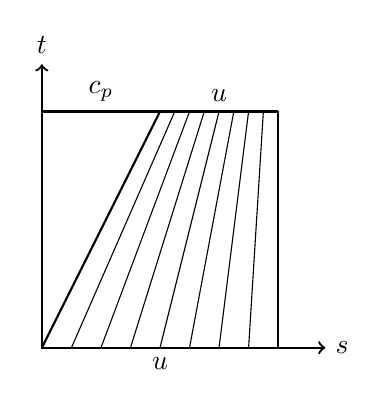
\begin{tikzpicture}[scale = 3]
    					% Draw axes
    					\draw [<->,thick] (0,1.2) node[above] {$t$}
        				|- (1.2,0) node[right] {$s$};
    					% Draw two intersecting lines
						\draw [thick] (0,0) -- (.5,1);
						\draw [thick] (0,1) -- (1,1);
						\draw [thick] (1,0) -- (1,1);

						\draw [thin] (.25,0) -- (.625,1);
						\draw [thin] (.125,0) -- (.5625,1);
					
						\draw [thin] (.5,0) -- (.75,1);
						\draw [thin] (.375,0) -- (.6875,1);
						\draw [thin] (.625,0) -- (.8125,1);
						\draw [thin] (.875,0) -- (.9375,1);
						\draw [thin] (.75,0) -- (.875,1);
					
					
						\draw (.5,0) node[below] {$u$};
						\draw (.25,1) node[above] {$c_p$};
						\draw (.75,1) node[above] {$u$};
					\end{tikzpicture}
					\caption{$u \simeq_{\partial I} c_p \ast u$.}
					\label{fig:unit_axiom}
				\end{subfigure}
				~
				\begin{subfigure}[b]{.3\textwidth}
					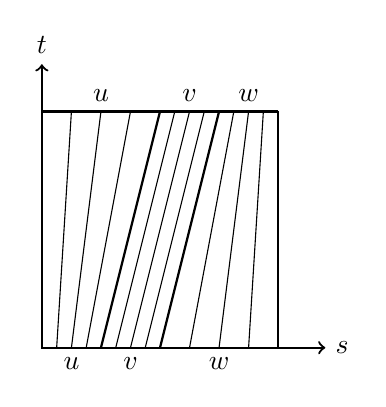
\begin{tikzpicture}[scale = 3]
    					% Draw axes
    					\draw [<->,thick] (0,1.2) node[above] {$t$}
        				|- (1.2,0) node[right] {$s$};
    					% Draw two intersecting lines
						\draw [thick] (.25,0) -- (.5,1);
						\draw [thick] (.5,0) -- (.75,1);
						\draw [thick] (0,1) -- (1,1);
						\draw [thick] (1,0) -- (1,1);
					
						\draw [thin] (.125,0) -- (.25,1);
						\draw [thin] (.0625,0) -- (.125,1);
						\draw [thin] (.1875,0) -- (.375,1);
					
						\draw [thin] (.375,0) -- (.625,1);
						\draw [thin] (.3125,0) -- (.5625,1);
						\draw [thin] (.4375,0) -- (.6875,1);

						\draw [thin] (.75,0) -- (.875,1);
						\draw [thin] (.625,0) -- (.8125,1);
						\draw [thin] (.875,0) -- (.9375,1);

						\draw (.125,0) node[below] {$u$};
						\draw (.375,0) node[below] {$v$};
						\draw (.75,0) node[below] {$w$};
					
						\draw (.25,1) node[above] {$u$};
						\draw (.625,1) node[above] {$v$};
						\draw (.875,1) node[above] {$w$};
					\end{tikzpicture}
					\caption{$(u \ast v) \ast w \simeq_{\partial I} u \ast (v \ast w)$.}
					\label{fig:associativity_axiom}
				\end{subfigure}
				~
				\begin{subfigure}[b]{.3\textwidth}
					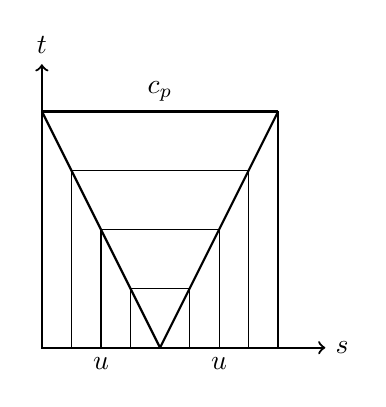
\begin{tikzpicture}[scale = 3]
    					% Draw axes
    					\draw [<->,thick] (0,1.2) node[above] {$t$}
        				|- (1.2,0) node[right] {$s$};
    					% Draw two intersecting lines
						\draw [thick] (0,1) -- (.5,0);
						\draw [thick] (.5,0) -- (1,1);
						\draw [thick] (0,1) -- (1,1);
						\draw [thick] (1,0) -- (1,1);

						\draw [thin] (.25,0) -- (.25,.5);
						\draw [thin] (.125,0) -- (.125,.75);				
						\draw [thin] (.375,0) -- (.375,.25);

						\draw [thin] (.625,0) -- (.625,.25);
						\draw [thin] (.875,0) -- (.875,.75);
						\draw [thin] (.75,0) -- (.75,.5);

						\draw [thin] (.25,.5) -- (.75,.5);
						\draw [thin] (.125,.75) -- (.875,.75);
						\draw [thin] (.375,.25) -- (.625,.25);
					
						\draw (.5,1) node[above] {$c_p$};
						\draw (.25,0) node[below] {$u$};
						\draw (.75,0) node[below] {$\wbar{u}$};
					\end{tikzpicture}
					\caption{$u \ast \wbar{u} \simeq_{\partial I} c_p$.}
					\label{fig:reverse_path}
				\end{subfigure}
				\caption{Visualization of the proof that $\Pi(X)$ is a grupoid object.}
			\end{figure}
			Similarly, considering figure \ref{fig:associativity_axiom} leads to $F \in \mathsf{Top}(I \times I,X)$ defined by
			\begin{equation*}
				F(s,t) := \ccases{
					\displaystyle u\del[3]{\frac{4s}{t + 1}} & -1 \leq 4s - 1 \leq t,\\
					\displaystyle v(4s - t - 1) & t \leq 4s - 1 \leq t + 1,\\
					\displaystyle w\del[3]{\frac{4s - t - 2}{4 - t - 2}} & t + 1 \leq 4s - 1 \leq 3.
				}
			\end{equation*}
			Lastly, we check that $\Pi(X)$ is a grupoid. To this end, for a path $u$ from $p$ to $q$, define its \bld{reverse path $\wbar{u}$} by
			\begin{equation*}
				\wbar{u}(s) := u(1 - s). 
			\end{equation*}
			We claim that $u \ast \wbar{u} \simeq_{\partial I} c_p$. From figure \ref{fig:reverse_path} we deduce that $F \in \mathsf{Top}(I \times I,X)$ is given by
			\begin{equation*}
				F(s,t) := \ccases{
					u(2s) & 0 \leq 2s \leq 1 - t,\\
					u(1 - t) & 1 - t \leq 2s \leq t + 1,\\
					\wbar{u}(2s - 1) & t + 1 \leq 2s \leq 2.
				}
			\end{equation*}
		\item \textit{Definition of $\Pi$ on morphisms.} Let $f \in \mathsf{Top}(X,Y)$. Then $\Pi(f)$ is a functor from $\Pi(X)$ to $\Pi(Y)$. Define $\Pi(f)$ as follows:
			\begin{itemize}[leftmargin = *]
				\item Let $p \in \ob\del[1]{\Pi(X)}$. Then define $\Pi(f)(p) := f(p) \in \ob\del[1]{\Pi(Y)}$.
				\item Let $\sbr{u} \in \Pi(X)(p,q)$. Then define $\Pi(f)\sbr{u} := \sbr[0]{f \circ u} \in $. We have to check that this definition is independent of the choice of the representative.

					\begin{lemma}
						Let $u$ and $v$ be paths from $p$ to $q$ in $X$ and suppose that $\sbr{u} = \sbr{v}$. Then for any $f \in \mathsf{Top}(X,Y)$ we also have that $\sbr[0]{f \circ u} = \sbr[0]{f \circ v}$.
					\end{lemma}

					\begin{proof}
						Suppose that $H : u \simeq_{\partial I} v$. Define $F \in \mathsf{Top}(I \times I,Y)$ by
						\begin{equation*}
							F(s,t) := (f \circ F)(s,t).
						\end{equation*}
						Then $F : f \circ u \simeq_{\partial I} f \circ v$.
					\end{proof}
			\end{itemize}
	\end{enumerate}
	Checking that $\Pi$ satisfies the functorial properties is left as an exercise.
\end{proof}

\begin{exercise}
	Check that $\Pi : \mathsf{Top} \to \mathsf{Grpd}$ is indeed a functor.
\end{exercise}

\subsection*{The Fundamental Group}

\begin{lemma}
	Let $\mathcal{\altG}$ be a locally small grupoid. Then for every $X \in \ob(\mathcal{\altG})$, $\mathcal{\altG}(X,X)$ can be equipped with a group structure.
	\label{lem:groupoid_group}
\end{lemma}

\begin{proof}
	Since $\mathcal{\altG}$ is locally small, $\mathcal{\altG}(X,X)$ is a set for every $X \in \ob(\mathcal{\altG})$. Define a multiplication $\mathcal{\altG}(X,X) \times \mathcal{\altG}(X,X) \to \mathcal{\altG}(X,X)$ by $gh := h \circ g$. Clearly, this multiplication is associative. Moreover, the identity element is given by $\id_X \in \mathcal{\altG}(X,X)$ and since every $g \in \mathcal{\altG}(X,X)$ is an isomorphism, the multiplicative inverse is given by the inverse in $\mathcal{\altG}(X,X)$. 
\end{proof}

\begin{proposition}
	There is a functor $\mathsf{Top}_\ast \to \mathsf{Grp}$.
\end{proposition}

\begin{proof}
	Define $\pi_1 : \mathsf{Top}_\ast \to \mathsf{Grp}$ on objects $(X,p) \in \mathsf{Top}_\ast$ by 
	\begin{equation*}
		\pi_1(X,p) := \Pi(X)(p,p).
	\end{equation*}
	By theorem \ref{thm:fundamental_groupoid} together with lemma \ref{lem:groupoid_group}, $\pi_1(X,p)$ is actually a group, called the \bld{fundamental group of $X$ with basepoint $p$}. On morphisms $f \in \mathsf{Top}_\ast\del[1]{(X,p),(Y,q)}$, define 
	\begin{equation*}
		\pi_1(f) := \Pi(f) : \Pi(X)(p,p) \to \Pi(Y)(q,q).
	\end{equation*}
	Let $\sbr{u},\sbr{v} \in \pi_1(X,p)$. Then 
	\begin{align*}
		\pi_1(\sbr{u}\sbr{v}) &= \Pi(f)(\sbr{u}\sbr{v})\\
		&= \Pi(f)\sbr{u \ast v}\\
		&= \sbr[0]{f \circ (u \ast v)}\\
		&= \sbr[0]{(f \circ u) \ast (f \circ v)}\\
		&= \Pi(f)\sbr{u} \Pi(f)\sbr{v}\\
		&= \pi_1(f)\sbr{u}\pi_1(f)\sbr{v}.
	\end{align*}
	Thus $\pi_1(f)$ is a morphism in $\mathsf{Grp}$. Functoriality of $\pi_1$ immediately follows from the functoriality of $\Pi$.
\end{proof}

\begin{lemma}
	Let $X \in \ob(\mathsf{Top})$, $p \in X$ and $A$ be the path component of $X$ containing $p$. Then $\pi_1(\iota)$, where $\iota : A \hookrightarrow X$ denotes the inclusion, is an isomorphism.
\end{lemma}

\begin{proof}
	Suppose $\sbr{u} \in \ker\pi_1(\iota)$. Then $\sbr{\iota \circ u} = \sbr[0]{c_p}$ and Hence $F : \iota \circ u \simeq_{\partial I} c_p$. Since $I \times I$ is path connected and $p \in F(I \times I)$, it follows that $F(I \times I) \subseteq A$ and thus $F : u \simeq_{\partial I} c_p$ in $A$ and hence $\sbr{u} = \sbr[0]{c_p}$. To see that $\pi_1(\iota)$ is surjective, just observe that $u(I) \subseteq A$ for $\sbr{u} \in \pi_1(X,p)$ since $u(I)$ is path connected and $p \in u(I)$.
\end{proof}

\begin{lemma}
	Let $X \in \ob(\mathsf{Top})$ be path connected and $p,q \in X$. Then 
	\begin{equation*}
		\pi_1(X,p) \cong \pi_1(X,q).	
	\end{equation*}
	\label{lem:fundamental_group_path_connected}
\end{lemma}

\begin{proof}
	Since $X$ is path connected we find a path $v$ from $p$ to $q$ in $X$. Define a mapping $\Phi_v : \pi_1(X,p) \to \pi_1(X,q)$ 
	\begin{equation*}
		\Phi_v\sbr{u} := \sbr{\wbar{v} \ast u \ast v}.
	\end{equation*}
	Clearly, $\Phi_v$ is invertible with inverse $\Phi_{\wbar{v}}$. Moreover, for $\sbr{u},\sbr{w} \in \pi_1(X,p)$ we have that
	\begin{align*}
		\Phi_v(\sbr{u}\sbr{w}) &= \Phi_v\sbr{u \ast w}\\
		&= \sbr[0]{\wbar{v} \ast u \ast w \ast v}\\
		&= \sbr[0]{\wbar{v} \ast u \ast v \ast \wbar{v} \ast w \ast v}\\
		&= \sbr[0]{\wbar{v} \ast u \ast v}\sbr[0]{\wbar{v} \ast w \ast v}\\
		&= \Phi_v\sbr{u}\Phi_v\sbr{w}.
	\end{align*}
\end{proof}

\subsection*{$\pi_1(\mathbb{S}^1)$}  

\begin{definition}[Exponential Quotient Map]
	The mapping $\varepsilon : \mathbb{R} \to \mathbb{S}^1$ defined by
	\begin{equation}
		\varepsilon(x) := e^{2\pi i x}
	\end{equation}
	\noindent is called the \bld{exponential quotient map}.
\end{definition}

\begin{proposition}[Lifting Property of the Circle]
	Let $n \in \mathbb{Z}$, $n \geq 0$, $X \subseteq \mathbb{R}^n$ compact and convex, $p \in X$, $f \in \mathsf{Top}_\ast\del[1]{(X,p),(\mathbb{S}^1,1)}$ and $m \in \mathbb{Z}$. Then there exists a unique map $\wtilde{f} \in \mathsf{Top}_\ast\del[1]{(X,p),(\mathbb{R},m)}$, called the \bld{lifting of $f$}, such that 
	\begin{equation*}
		\centering
		\xymatrix{
			& (\mathbb{R},m) \ar[d]^\varepsilon\\
			(X,p) \ar[r]_f\ar[ur]^{\wtilde{f}}	& (\mathbb{S}^1,1)
		}
		\end{equation*}
		\noindent commutes. 
		\label{prop:lifting_circle}
	\end{proposition}

\begin{proof}
	We show first existence and then uniqueness.
	\begin{enumerate}[label = \textit{Step \arabic*:},wide = 0pt, itemsep = 1.5ex]
		\item \textit{Existence.} Since $X$ is compact and $f$ is continuous, $f$ is uniformly continuous on $X$. Thus we find $\delta > 0$ such that $\abs{f(x) - f(y)} < 2$, whenever $\abs{x - y} < \delta$, i.e. $f(x)$ and $f(y)$ are not antipodal points. Moreover, since $X$ is compact, $X$ is bounded and hence we find $N \in \mathbb{N}$, such that $\abs{x - y} < N\delta$ holds for all $x,y \in X$. Let $x \in X$. For $0 \leq k \leq N$, define $L_k : X \to X$ by
			\begin{equation*}
				L_k(x) := \del[3]{1 - \frac{k}{N}}p + \frac{k}{N}x.
			\end{equation*}
		Those are well defined functions since $X$ is convex. Moreover, each $L_k$ is continuous. Indeed, it is easy to check that $L_k$ is Lipschitz. Also, for each $0 \leq k < N$, $f\del[0]{L_k(x)}$ and $f\del[0]{L_{k + 1}(x)}$ are not antipodal for all $x \in X$. Indeed, it is easy to check that $\abs[0]{L_k(x) - L_{k + 1}(x)} < \delta$ holds for all $x \in X$. For $0 \leq k < N$ define $g_k : X \to \mathbb{S}^1 \setminus \cbr{-1}$ by
			\begin{equation*}
				g_k(x) := \frac{f(L_{k + 1}(x))}{f(L_k(x))}.
			\end{equation*}
		Clearly $g_k$ is well defined and continuous as a composition of continuous functions. Let $\Log : \mathbb{S}^1 \setminus \cbr{-1} \to \mathbb{C}$ denote the principal branch of the logarithm. Define $\wtilde{f} : X \to \mathbb{R}$ by
			\begin{equation*}
				\wtilde{f}(x) := m + \frac{1}{2\pi i} \sum_{k = 0}^{N - 1} \Log(g_k(x)).
			\end{equation*}
		Clearly, $\wtilde{f}$ is continuous and moreover we have that $\wtilde{f} = m$ since $g_k(p) = 1$ for all $0\leq k < N$. Finally, for any $x \in X$ we have that
			\begin{equation*}
				(\varepsilon \circ \wtilde{f})(x) = \varepsilon(m)\prod_{k = 0}^{N - 1} g_k(x) = \frac{f(L_N(x))}{f(L_0(x))} = \frac{f(x)}{f(p)} = f(x). 
			\end{equation*}
		\item \textit{Uniqueness.} Suppose $\wtilde{g} \in \mathsf{Top}_\ast\del[1]{(X,p),(\mathbb{R},m)}$ is another such function. Define $\varphi \in \mathsf{Top}_\ast\del[1]{(X,p),(\mathbb{R},0)}$ by
			\begin{equation*}
				\varphi(x) := \wtilde{f}(x) - \wtilde{g}(x).
			\end{equation*}
		Then clearly $\varepsilon \circ \varphi = 1$ and thus $\varphi(X) \subseteq \mathbb{Z}$. Since $X$ is convex, $X$ is connected and so $\varphi = 0$.
	\end{enumerate}
\end{proof}

\begin{corollary}
	Let $u,v \in \Omega(\mathbb{S}^1,1)$ such that $\sbr{u} = \sbr{v}$. If $\wtilde{u},\wtilde{v} : (I,0) \to (\mathbb{R},0)$ are the liftings of $u$ and $v$, respectively, then $\sbr[0]{\wtilde{u}} = \sbr[0]{\wtilde{v}}$.
	\label{cor:degree}
\end{corollary}

\begin{proof}
	Let $F : u \simeq_{\partial I} v$. By proposition \ref{prop:lifting_circle}, we find $\wtilde{F} \in \mathsf{Top}_\ast\del[1]{(I \times I, (0,0)),(\mathbb{R},0)}$, such that $\varepsilon \circ \wtilde{F} = F$. We claim that $\wtilde{F} : \wtilde{u} \simeq_{\partial I} \wtilde{v}$. For $s \in I$ define $\wtilde{u}_0(s) := \wtilde{F}(s,0)$. Then $\wtilde{u}_0(0) = \wtilde{F}(0,0) = 0$ and since $\wtilde{u}_0$ is continuous we have that $\wtilde{u}_0 \in \mathsf{Top}_\ast\del[1]{(I,0),(\mathbb{R},0)}$. Moreover
	\begin{equation*}
		(\varepsilon \circ \wtilde{u}_0)(s) = \varepsilon\del[1]{\wtilde{F}(s,0)} = F(s,0) = u(s)
	\end{equation*}
	\noindent for all $s \in I$ and thus $\wtilde{u}_0$ is a lifting of $u$. But by proposition \ref{prop:lifting_circle}, liftings are unique and thus $\wtilde{u}_0 = \wtilde{u}$. Next define $\wtilde{w}_0(t) := \wtilde{F}(0,t)$ for all $t \in I$. Then $\wtilde{w}_0(0) = \wtilde{F}(0,0) = 0$ and so $\wtilde{w}_0 \in \mathsf{Top}_\ast\del[1]{(I,0),(\mathbb{R},0)}$. Moreover
	\begin{equation*}
		(\varepsilon \circ \wtilde{w}_0)(t) = \varepsilon\del[1]{\wtilde{F}(0,t)} = F(0,t) = u(0) = v(0) = 1.
	\end{equation*}
	\noindent for all $t \in I$. Thus
	\begin{equation*}
		\centering
		\xymatrix{
			& (\mathbb{R},0) \ar[d]^\varepsilon\\
			(I,0) \ar[r]_{c_1}\ar[ur]^{\wtilde{w}_0} & (\mathbb{S}^1,1)
		}
	\end{equation*}
	\noindent commutes. But also $c_0$ makes the above diagram commute. By uniqueness, $\wtilde{w}_0 = c_0$. Define $\wtilde{v}_0(s) := \wtilde{F}(s,1)$ for all $s \in I$. Then $\wtilde{v}_0(0) = \wtilde{F}(0,1) = \wtilde{w}_0(1) = 0$ and it is easy to check that $\wtilde{v}_0$ is a lift for $v$. Hence $\wtilde{v}_0 = \wtilde{v}$. Finally, define $\wtilde{w}_1(t) := \wtilde{F}(1,t)$ for all $t \in I$. Then $\wtilde{w}_1(0) = \wtilde{F}(1,0) = \wtilde{u}(1)$ and thus $\wtilde{w}_1 \in \mathsf{Top}_\ast\del[1]{(I,0),(\mathbb{R},\wtilde{u}(0))}$. Moreover
	\begin{equation*}
		(\varepsilon \circ \wtilde{w}_1)(t) = \varepsilon\del[1]{\wtilde{F}(1,t)} = F(1,t) = v(1) = u(1) = 1
	\end{equation*}
	\noindent for all $t \in I$. By proposition \ref{prop:lifting_circle}, we have again that $\wtilde{w}_1 = c_{\wtilde{u}(1)}$. So $F : \wtilde{u} \simeq_{\partial I} \wtilde{v}$.
\end{proof}

\begin{definition}[Degree]
	Let $u \in \Omega(\mathbb{S}^1,1)$. The \bld{degree of $u$}, written $\deg u$, is defined by $\deg u := \wtilde{u}(1)$, where $\wtilde{u}$ is the unique lift of $u$ such that $\wtilde{u}(0) = 0$. 
\end{definition}

\begin{theorem}[Fundamental Group of the Circle]
	$\pi_1(\mathbb{S}^1) \cong \mathbb{Z}$.
\end{theorem}

\begin{proof}
	Define $\deg : \pi_1(\mathbb{S}^1,1) \to \mathbb{Z}$ by $\deg \sbr{u} := \deg u$. This is well defined by corollary \ref{cor:degree}, since if $\sbr{u} = \sbr{v}$, then $\sbr[0]{\wtilde{u}} = \sbr[0]{\wtilde{v}}$ and in particular $\wtilde{u}(1) = \wtilde{v}(1)$. 
	\begin{enumerate}[label = \textit{Step \arabic*:},wide = 0pt, itemsep = 1.5ex]
		\item \textit{$\deg \in \mathsf{Grp}\del[1]{\pi_1(\mathbb{S}^1,1),(\mathbb{Z},+)}$.} Let $\sbr{u},\sbr{v} \in \pi_1(\mathbb{S}^1,1)$ and $m := \deg\sbr{u}$, $n := \deg \sbr{v}$. Moreover, let $\wtilde{u}$ and $\wtilde{v}$ denote the unique liftings of $u$ and $v$, respectively, such that $\wtilde{u}(0) = 0$ and $\wtilde{v}(0) = 0$. Define
			\begin{equation*}
				\wtilde{w}(s) := \ccases{
				\wtilde{u}(2s) & 0 \leq s \leq \frac{1}{2},\\
				m + \wtilde{v}(2s - 1) & \frac{1}{2} \leq s \leq 1.
			}
			\end{equation*}
		Clearly $\wtilde{w}$ is continuous and $\wtilde{w}(0) = 0$. Hence $\wtilde{w} \in \mathsf{Top}_\ast\del[1]{(I,0),(\mathbb{R},0)}$. Also we have that $\varepsilon \circ \wtilde{w} = u \ast v$ and thus $\wtilde{w}$ is the lift of $u \ast v$. But $\wtilde{w}(1) = m + n$ and so
			\begin{equation*}
				\deg(\sbr{u}\sbr{v}) = \deg\sbr{u\ast v} = \deg (u \ast v) = \wtilde{w}(1) = m + n = \deg\sbr{u} + \deg \sbr{v}.
			\end{equation*}
		\item \textit{$\deg$ is injective.} Suppose $\deg\sbr{u} = 0$. Then $\wtilde{u}(1) = 0$ and thus $\wtilde{u} \in \Omega(\mathbb{R},0)$. Since $\mathbb{R}$ is contractible, we have that $\sbr[0]{\wtilde{u}} = \sbr{c_0}$ and thus
			\begin{equation*}
				\sbr{u} = \sbr[0]{\varepsilon \circ \wtilde{u}} = \pi_1(\varepsilon)\sbr[0]{\wtilde{u}} = \pi_1(\varepsilon)\sbr{c_0} = \sbr{c_1}.
			\end{equation*}
			Thus $\ker(\deg)$ is trivial.
		\item \textit{$\deg$ is surjective.} Let $m \in \mathbb{Z}$. Then
			\begin{equation*}
				\deg\sbr[0]{\varepsilon^m} = \deg \varepsilon^m = \wwtilde{\varepsilon^m}(1) = m.
			\end{equation*}
	\end{enumerate}
\end{proof}

\section*{The Seifert-Van Kampen Theorem}
\subsection*{Coproducts and Pushouts in $\mathsf{Grp}$}

\begin{proposition}[Coproducts in $\mathsf{Grp}$]
	$\mathsf{Grp}$ has all small coproducts.
\end{proposition}

\begin{proof}
	Let $A \in \ob(\mathsf{Set})$ and $\mathsf{A}$ be the small category defined as the discrete category with $\ob(\mathsf{A}) := A$, i.e.
	\begin{equation*}
		\xymatrix{
			\bullet & \bullet & \bullet & \cdots & \bullet & \bullet & \bullet
		}
	\end{equation*}	
	Let $D : \mathsf{A} \to \mathsf{Grp}$ be a functor. Hence we get a family $(G_\alpha)_{\alpha \in A}$ in $\mathsf{Grp}$, where $G_\alpha := D(\alpha)$ for all $\alpha \in A$. A \bld{word} in $(G_\alpha)_{\alpha \in A}$ is a finite sequence in $\coprod_{\alpha \in A}G_\alpha$. A word in $(G_\alpha)_{\alpha \in A}$ will simply be written as $(g_1,\dots, g_n)$, where $g_k \in G_\alpha$ for some $\alpha \in A$. The \bld{empty word} is denoted by $()$. Let $\mathcal{W}$ denote the set of all words in $(G_\alpha)_{\alpha \in A}$. On $\mathcal{W}$ define a multiplication by \bld{concatenation}
	\begin{equation*}
		(g_1,\dots, g_n)(h_1,\dots, h_m) := (g_1, \dots, g_n,h_1, \dots, h_m).
	\end{equation*}
	An \bld{elementary reduction} is an operation of one of the following forms:
	\begin{itemize}[leftmargin = *]
		\item $(g_1, \dots ,g_k,g_{k + 1}, \dots, g_n) \mapsto (g_1,\dots,g_kg_{k + 1},\dots,g_n $, where $g_k,g_{k + 1} \in G_\alpha$ for some $\alpha \in A$.
		\item $(g_1,\dots,g_{k - 1},1_\alpha,g_{k + 1},\dots,g_n) \mapsto (g_1,\dots,g_{k - 1},g_{k + 1},\dots,g_n)$.
	\end{itemize}
	Let $\sim$ denote the equivalence relation on $\mathcal{W}$ generated by elementary reductions. 
	
	\begin{lemma}
		$\mathcal{W}/{\sim}$ together with concatenation of representatives is an element of $\mathsf{Grp}$.
		\label{lem:free_product}
	\end{lemma}

	\begin{proof}
		Define
		\begin{equation*}
			\sbr[0]{(g_1,\dots,g_n)}\sbr[0]{(h_1,\dots,h_m)} := \sbr[0]{(g_1,\dots,g_n,h_1,\dots,h_m)}.
		\end{equation*}
		It is left to the reader to show that this is well defined and that $\mathcal{W}/{\sim}$ is indeed a group.
	\end{proof}

	The group defined in lemma \ref{lem:free_product} will be denoted by $\bigast_{\alpha \in A}G_\alpha$ and called the \bld{free product of $(G_\alpha)_{\alpha \in A}$}. Let us define a cocone on $D$. For this consider the inclusions $\iota_\alpha : G_\alpha \to \bigast_{\alpha \in A}G_\alpha$ defined by
	\begin{equation*}
		\iota_\alpha(g) := \sbr[0]{(g)}
	\end{equation*}
	\noindent for all $\alpha \in A$. It is immediate from
	\begin{equation*}
		\iota_\alpha(gh) = \sbr[0]{(gh)} = \sbr[0]{(g,h)} = \sbr[0]{(g)}\sbr[0]{(h)} = \iota_\alpha(g)\iota_\alpha(h)
	\end{equation*}
	\noindent for $g,h \in G_\alpha$, that $\iota_\alpha$ is a morphism of groups. Since there are only the identity morphisms in $\mathsf{A}$, $\del[1]{\bigast_{\alpha \in A}G_\alpha, (\iota_\alpha)_{\alpha \in A}}$ is a cocone on $D$. Let us show that this is in fact a universal cocone. To this end, suppose that $\del[1]{C,(\varphi_\alpha)_{\alpha \in A}}$ is another cocone on $D$. Define a mapping $\wbar{f} : \bigast_{\alpha \in A}G_\alpha \to C$ by
	\begin{equation*}
		\wbar{f}\sbr[0]{(g_1,\dots,g_n)} := \varphi_{\alpha_1}(g_1)\cdots \varphi_{\alpha_n}(g_n)
	\end{equation*}
	\noindent where $g_k \in G_{\alpha_k}$. Then $\wbar{f}$ is easily seen to be well defined since each $\varphi_\alpha$ is  a morphism of groups. Moreover, if $g \in G_\alpha$, then
	\begin{equation*}
		(\wbar{f} \circ \iota_\alpha)(g) = \wbar{f}\sbr[0]{(g)} = \varphi_\alpha(g)
	\end{equation*}
	\noindent for all $\alpha \in A$. Suppose that $f : \bigast_{\alpha \in A}G_\alpha \to C$ is another homomorphism of groups such that $f \circ \iota_\alpha = \varphi_\alpha$ for all $\alpha \in A$. Then for $\sbr[0]{(g_1,\dots,g_n)} \in \bigast_{\alpha \in A} G_\alpha$ we have
	\begin{align*}
		f\sbr[0]{(g_1,\dots,g_n)} &= f(\sbr[0]{(g_1)} \cdots \sbr[0]{(g_n)})\\
		&= f\sbr[0]{(g_1)} \cdots f\sbr[0]{(g_n)}\\
		&= f\del[0]{\iota_{\alpha_1}(g_1)} \cdots f\del[0]{\iota_{\alpha_n}(g_n)}\\
		&= \varphi_{\alpha_1}(g_1)\cdots \varphi_{\alpha_n}(g_n)\\
		&= \wbar{f}\sbr[0]{(g_1,\dots,g_n)}.
	\end{align*}
\end{proof}

\begin{exercise}
	Check that $\mathcal{W}/{\sim}$ is indeed a group with the declared group structure and that $\wbar{f}$ is indeed well defined.
\end{exercise}

\begin{proposition}[Pushouts in $\mathsf{Grp}$]
	$\mathsf{Grp}$ has all pushouts.	
\end{proposition}

\begin{proof}
	Consider the diagram $D : \mathsf{A} \to \mathsf{Grp}$
	\begin{equation*}
		\xymatrix@R=0pc{
			\bullet \ar[r]\ar[dd] & \bullet & & G \ar[r]^{\varphi_1}\ar[dd]_{\varphi_2} & H_1\\
			& & \xrightarrow{D}\\
			\bullet & & & H_2
		}
	\end{equation*}
\end{proof}
